% !TeX root = booklet-03.tex
\clearpage
\subsection{سطوح منطقی و \lr{Noise Margin}}
\label{sec:noise-margin}
خروجی یک گیت، ورودی گیت بعدی را تغذیه می‌کند. برای انتقال صحیح
داده، بازه ولتاژ تولیدشده در خروجی باید در بازه معتبر ورودی گیت
گیرنده قرار گیرد. نویز می‌تواند ولتاژ دریافتی را تغییر دهد.
\lr{Noise Margin} مقدار تغییر نامطلوبی را توصیف می‌کند که این
سازگاری را در شرایط تعریف‌شده حفظ می‌کند
\cite[بخش \secnum{۲.۵.۳}، صفحات ۹۱ و ۹۲]{weste}
\cite[اسلایدهای ۹ و ۱۰]{dcslides}.

\subsubsection{تعریف چهار سطح ولتاژ}
\label{sec:noise-logic-levels}
برای ورودی، \(V_{\mathrm{IL}}\) بیشترین ولتاژ پذیرفته‌شده به‌عنوان
\lr{LOW} و \(V_{\mathrm{IH}}\) کمترین ولتاژ پذیرفته‌شده به‌عنوان
\lr{HIGH} است. برای خروجی، \(V_{\mathrm{OL}}\) بیشترین ولتاژ
تولیدشده در حالت \lr{LOW} و \(V_{\mathrm{OH}}\) کمترین ولتاژ
تولیدشده در حالت \lr{HIGH} است. حرف \lr{I} به ورودی، حرف
\lr{O} به خروجی و حرف‌های \lr{L} و \lr{H} به سطح پایین و بالا
اشاره می‌کنند. جدول \ref{tab:noise-level-definitions} تعریف‌ها
را به شکل بازه نشان می‌دهد \cite[صفحه ۹۱]{weste}.
\begin{table}[!htbp]
\centering
\small
\caption{بازه‌های منطقی برای ولتاژهای بین زمین و تغذیه.
مرزهای ورودی به گیرنده و مرزهای خروجی به فرستنده مربوط‌اند.}
\label{tab:noise-level-definitions}
\begin{tabularx}{\linewidth}{cc>{\raggedleft\arraybackslash}X}
\toprule
پایانه & حالت & بازه معتبر\\
\midrule
ورودی & \lr{LOW} & \(0\le V_{\mathrm{in}}\le V_{\mathrm{IL}}\)\\
ورودی & \lr{HIGH} & \(V_{\mathrm{IH}}\le V_{\mathrm{in}}\le V_{DD}\)\\
خروجی & \lr{LOW} & \(0\le V_{\mathrm{out}}\le V_{\mathrm{OL}}\)\\
خروجی & \lr{HIGH} & \(V_{\mathrm{OH}}\le V_{\mathrm{out}}\le V_{DD}\)\\
\bottomrule
\end{tabularx}
\end{table}

بازه \(V_{\mathrm{IL}}<V_{\mathrm{in}}<V_{\mathrm{IH}}\) را
\lr{Indeterminate Region} یا \lr{Forbidden Zone} می‌نامند.
در این بازه، مشخصات منطقیِ تعریف‌شده، تفسیر معتبر صفر یا یک را
تضمین نمی‌کنند. مدار همچنان ولتاژ و جریان فیزیکی دارد و می‌توان
آن را با مشخصه انتقال تحلیل کرد.
\(V_{\mathrm{inv}}\) نیز نقطه \(V_{\mathrm{out}}=V_{\mathrm{in}}\)
از بخش \ref{sec:inverter-input-threshold} است. دو مرز
\(V_{\mathrm{IL}},V_{\mathrm{IH}}\) با معیار جداگانه‌ای تعیین
می‌شوند که در ادامه استخراج می‌شود.

در شرایط سازگار معمول، خروجی پایین باید از حداکثر ورودی پایین
کمتر و خروجی بالا باید از حداقل ورودی بالا بیشتر باشد. شکل
\ref{fig:noise-level-ranges} فاصله‌های مربوط را نشان می‌دهد.
\begin{figure}[!htbp]
\centering
\begin{latin}
\PersianMathDigits
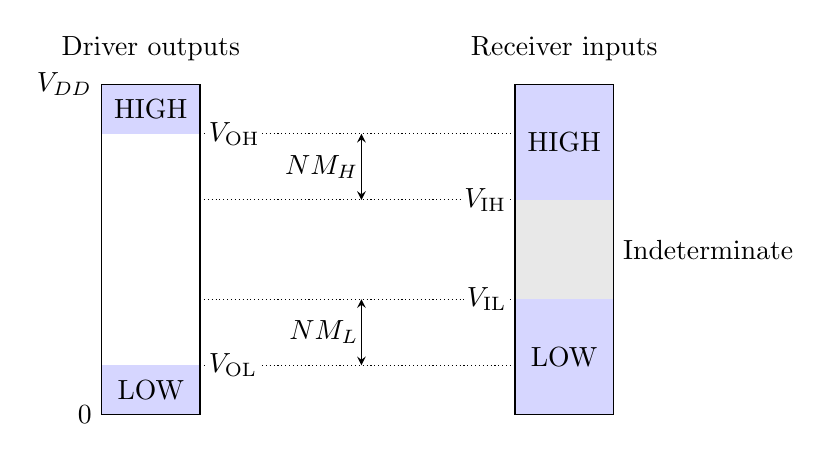
\begin{tikzpicture}[x=1cm,y=4.2cm,>=stealth]
\fill[blue!16] (0,0) rectangle (1.25,0.15);
\fill[blue!16] (0,0.85) rectangle (1.25,1);
\draw (0,0) rectangle (1.25,1);
\fill[blue!16] (5.25,0) rectangle (6.5,0.35);
\fill[gray!18] (5.25,0.35) rectangle (6.5,0.65);
\fill[blue!16] (5.25,0.65) rectangle (6.5,1);
\draw (5.25,0) rectangle (6.5,1);
\foreach \y in {0.15,0.35,0.65,0.85}
 {\draw[densely dotted] (1.25,\y)--(5.25,\y);}
\node[above] at (0.625,1.04) {Driver outputs};
\node[above] at (5.875,1.04) {Receiver inputs};
\node[left] at (0,0) {\(0\)};
\node[left] at (0,1) {\(V_{DD}\)};
\node at (0.625,0.075) {LOW};
\node at (0.625,0.925) {HIGH};
\node at (5.875,0.175) {LOW};
\node at (5.875,0.825) {HIGH};
\node[right] at (6.5,0.5) {Indeterminate};
\node[anchor=west,fill=white,inner sep=1pt] at (1.32,0.15) {\(V_{\mathrm{OL}}\)};
\node[anchor=west,fill=white,inner sep=1pt] at (1.32,0.85) {\(V_{\mathrm{OH}}\)};
\node[anchor=east,fill=white,inner sep=1pt] at (5.18,0.35) {\(V_{\mathrm{IL}}\)};
\node[anchor=east,fill=white,inner sep=1pt] at (5.18,0.65) {\(V_{\mathrm{IH}}\)};
\draw[<->] (3.3,0.15)--(3.3,0.35)
 node[midway,left,fill=white,inner sep=1pt] {\(NM_L\)};
\draw[<->] (3.3,0.65)--(3.3,0.85)
 node[midway,left,fill=white,inner sep=1pt] {\(NM_H\)};
\end{tikzpicture}
\end{latin}
\caption{طرح آموزشی بازه‌های ورودی و خروجی بر اساس شکل
\secnum{۲.۲۹} کتاب و اسلاید ۹. فاصله‌ها شماتیک‌اند و مقیاس
عددی یک فناوری را نمایش نمی‌دهند.}
\label{fig:noise-level-ranges}
\end{figure}

\subsubsection{استخراج حاشیه نویز از شرط سازگاری}
\label{sec:noise-margin-definition}
برای حالت پایین، بدترین خروجی مجاز فرستنده
\(V_{\mathrm{OL}}\) است. اگر نویز نامطلوب مثبت با بزرگی
\(v_n\ge0\) به آن اضافه شود، ولتاژ دریافتی در این حالت
\(V_{\mathrm{OL}}+v_n\) می‌شود. برای باقی‌ماندن در بازه
\lr{LOW} گیرنده، باید
\begin{equation*}
 V_{\mathrm{OL}}+v_n\le V_{\mathrm{IL}}
 \quad\Longrightarrow\quad
 v_n\le V_{\mathrm{IL}}-V_{\mathrm{OL}}.
\end{equation*}
پس رابطه \secnum{۲.۵۸} کتاب چنین تعریف می‌شود
\begin{equation}
 \boxed{NM_L=V_{\mathrm{IL}}-V_{\mathrm{OL}}}.
 \label{eq:noise-low-margin}
\end{equation}
برای حالت بالا، بدترین خروجی مجاز
\(V_{\mathrm{OH}}\) است. نویز نامطلوب، ولتاژ را کاهش می‌دهد.
شرط باقی‌ماندن ورودی در بازه \lr{HIGH} برابر است با
\begin{equation*}
 V_{\mathrm{OH}}-v_n\ge V_{\mathrm{IH}}
 \quad\Longrightarrow\quad
 v_n\le V_{\mathrm{OH}}-V_{\mathrm{IH}}.
\end{equation*}
در نتیجه، رابطه \secnum{۲.۵۹} کتاب چنین است
\begin{equation}
 \boxed{NM_H=V_{\mathrm{OH}}-V_{\mathrm{IH}}}.
 \label{eq:noise-high-margin}
\end{equation}
هر دو حاشیه واحد ولت دارند. وقتی بزرگی نویز در هر دو حالت
مهم باشد، کمیت \(\min(NM_L,NM_H)\) حاشیه محدودکننده را
نشان می‌دهد. مقدار صفر، فاصله اطمینان اضافی باقی نمی‌گذارد.
مقدار منفی یعنی حتی بدون نویز اضافه، همه خروجی‌های مجاز
فرستنده در بازه معتبر گیرنده قرار نمی‌گیرند.

\paragraph*{مثال آموزشی ارتباط دو گیت}
فرض کنید فرستنده \(V_{\mathrm{OL}}=\qty{0.1}{\volt}\) و
\(V_{\mathrm{OH}}=\qty{0.9}{\volt}\) و گیرنده
\(V_{\mathrm{IL}}=\qty{0.3}{\volt}\) و
\(V_{\mathrm{IH}}=\qty{0.7}{\volt}\) داشته باشند.
هر دو حاشیه \(\qty{0.2}{\volt}\) هستند.
نویز مثبت \(\qty{0.15}{\volt}\) روی بدترین سطح پایین،
ورودی \(\qty{0.25}{\volt}\) می‌دهد که هنوز معتبر است.
نویز کاهنده با همین بزرگی روی بدترین سطح بالا،
\(\qty{0.75}{\volt}\) می‌دهد که آن هم معتبر است.
اما با نویز مثبت \(\qty{0.25}{\volt}\)، سطح پایین به
\(\qty{0.35}{\volt}\) می‌رسد و وارد بازه نامعین می‌شود.
در این حالت، تضمین مشخصات منطقی از بین می‌رود. مقدار خروجی
واقعی باید از مشخصه گیرنده تعیین شود.

\subsubsection{معنای \lr{Unity Gain} و بدترین خروجی مجاز}
\label{sec:noise-unity-gain}
شیب مشخصه را با \(g\) نشان می‌دهیم. تعریف مشتق و تقریب تغییر کوچک
ورودی در همسایگی یک نقطه چنین‌اند.
\[
 g=\frac{\mathrm{d}V_{\mathrm{out}}}{\mathrm{d}V_{\mathrm{in}}},\qquad
 \Delta V_{\mathrm{out}}\approx g\Delta V_{\mathrm{in}}.
\]
مثلاً در \(g=-0.3\)، تغییر ورودی
\(\qty{10}{\milli\volt}\)، تقریباً
\(-\qty{3}{\milli\volt}\) تغییر خروجی ایجاد می‌کند.
در \(g=-4\)، همان تغییر ورودی حدود
\(-\qty{40}{\milli\volt}\) تغییر خروجی می‌دهد.
علامت منفی، رفتار معکوس‌کننده و بزرگی شیب، نسبت بزرگی تغییرها
را نشان می‌دهد.

نزدیک دو ریل، معمولاً \(|g|<1\) و در بخش میانی گذار،
\(|g|>1\) است. در قرارداد کتاب و اسلاید ۱۰، دو نقطه مرزی
با شرط زیر تعیین می‌شوند
\begin{equation}
 \boxed{g=-1}.
 \label{eq:noise-unity-condition}
\end{equation}
واژه \lr{Unity} به بزرگی یک اشاره دارد. چون مشخصه
\lr{Inverter} کاهشی است، مقدار علامت‌دار شیب منفی یک است.
نقطه سمت چپ، \(V_{\mathrm{IL}}\) و نقطه سمت راست،
\(V_{\mathrm{IH}}\) را مشخص می‌کند.
کتاب این مرزبندی را کرانی محافظه‌کارانه برای بدترین حاشیه نویز
ایستا توصیف می‌کند \cite[شکل \secnum{۲.۳۰} و صفحه ۹۲]{weste}.

در شاخه بالای یک مشخصه کاهشی، بیشترین ورودی پایین مجاز،
کمترین خروجی بالا را می‌دهد. در شاخه پایین، کمترین ورودی بالا
مجاز، بیشترین خروجی پایین را می‌دهد. بنابراین، برای همین
قرارداد سطوح منطقی می‌نویسیم
\begin{equation}
 V_{\mathrm{OH}}=V_{\mathrm{out}}(V_{\mathrm{IL}}),\qquad
 V_{\mathrm{OL}}=V_{\mathrm{out}}(V_{\mathrm{IH}}).
 \label{eq:noise-output-levels}
\end{equation}
در دو نقطه مرزی، خروجی می‌تواند کمی از ریل متناظر فاصله داشته
باشد. کتاب این انتقال اثر ورودی به خروجی را
\lr{Noise Feedthrough} یا \lr{Propagated Noise} می‌نامد
\cite[صفحه ۹۲]{weste}. این افت باید در تفاضل حاشیه‌ها لحاظ شود.

شکل \ref{fig:noise-unity-vtc} یک مثال آموزشی متقارن با
\(V_t=0.1V_{DD}\) است. روابط مدل مربعی بخش‌های قبل برای رسم
آن به کار رفته‌اند. در این مثال،
\(V_{\mathrm{IL}}=0.4V_{DD}\)،
\(V_{\mathrm{IH}}=0.6V_{DD}\)،
\(V_{\mathrm{OH}}=0.9V_{DD}\) و
\(V_{\mathrm{OL}}=0.1V_{DD}\) هستند.
\begin{figure}[!htbp]
\centering
\begin{latin}
\PersianMathDigits
\begin{tikzpicture}[x=8.4cm,y=5cm,>=stealth]
\draw[->] (0,0)--(1.1,0) node[right] {\(V_{\mathrm{in}}/V_{DD}\)};
\draw[->] (0,0)--(0,1.12) node[above] {\(V_{\mathrm{out}}/V_{DD}\)};
\draw[thick,blue] (0,1)--(0.1,1);
\draw[thick,blue,domain=0.1:0.5,samples=110]
 plot (\x,{\x+0.1+sqrt(max(0,(1-2*\x)*0.8))})--(0.5,0.6);
\draw[thick,blue] (0.5,0.6)--(0.5,0.4);
\draw[thick,blue,domain=0.5:0.9,samples=110]
 plot (\x,{\x-0.1-sqrt(max(0,(2*\x-1)*0.8))});
\draw[thick,blue] (0.9,0)--(1,0);
\draw[densely dotted] (0.4,0)--(0.4,0.9)--(0,0.9);
\draw[densely dotted] (0.6,0)--(0.6,0.1)--(0,0.1);
\draw[thick,red] (0.34,0.96)--(0.46,0.84);
\draw[thick,red] (0.54,0.16)--(0.66,0.04);
\fill (0.4,0.9) circle[radius=1.7pt];
\fill (0.6,0.1) circle[radius=1.7pt];
\node[below] at (0.4,0) {\(V_{\mathrm{IL}}/V_{DD}\)};
\node[below] at (0.6,0) {\(V_{\mathrm{IH}}/V_{DD}\)};
\node[below] at (1,0) {\(1\)};
\node[left] at (0,0.9) {\(V_{\mathrm{OH}}/V_{DD}\)};
\node[left] at (0,0.1) {\(V_{\mathrm{OL}}/V_{DD}\)};
\node[left] at (0,1) {\(1\)};
\node[above right] at (0.65,0.65) {\(g=-1\)};
\end{tikzpicture}
\end{latin}
\caption{نقاط \lr{Unity Gain} در مثال فرضی
\(V_t/V_{DD}=0.1\). پاره‌خط‌های قرمز مماس‌های با شیب منفی یک
در مختصات نرمال‌شده‌اند. ساخت شکل بر اساس شکل \secnum{۲.۳۰}
کتاب و اسلاید ۱۰ است.}
\label{fig:noise-unity-vtc}
\end{figure}

\subsubsection{پیش‌نیاز مشتق‌گیری و استخراج شیب دو شاخه}
\label{sec:noise-derivatives}
برای استخراج تحلیلی، مدل متقارن
\(\beta_n=\beta_p\)، \(V_{tn}=V_{TP}=V_t>0\) و
\(V_{DD}>2V_t\) را به کار می‌بریم. آستانه و \lr{Mobility}
ثابت و اثرهای نشتی و \lr{CLM} صفر فرض می‌شوند.
کمیت مثبت \(K=V_{DD}-2V_t\) را با واحد ولت تعریف می‌کنیم.
برای کوتاه‌شدن محاسبه، \(x=V_{\mathrm{in}}\) و
\(y=V_{\mathrm{out}}\) می‌گذاریم. روابط شاخه‌های \lr{B} و
\lr{D} از \eqref{eq:inverter-b-transfer} و
\eqref{eq:inverter-d-transfer} هستند.

مشتق یک مقدار ثابت نسبت به \(x\) صفر و مشتق خود \(x\) یک است.
برای ریشه، اگر \(z=\sqrt{u}>0\)، آنگاه \(z^2=u\).
مشتق‌گیری دو طرف نسبت به \(u\) می‌دهد
\[
 2z\frac{\mathrm{d}z}{\mathrm{d}u}=1
 \quad\Longrightarrow\quad
 \frac{\mathrm{d}\sqrt{u}}{\mathrm{d}u}=\frac{1}{2\sqrt{u}}.
\]
وقتی \(u\) خودش تابع \(x\) است، نرخ تغییر بیرونی را در نرخ
تغییر درونی ضرب می‌کنیم. این همان \lr{Chain Rule} است
\begin{equation}
 \frac{\mathrm{d}\sqrt{u(x)}}{\mathrm{d}x}
 =\frac{1}{2\sqrt{u(x)}}\frac{\mathrm{d}u}{\mathrm{d}x},
 \qquad u(x)>0.
 \label{eq:noise-chain-rule}
\end{equation}
این رابطه در شاخه‌های باز و دور از رادیکال صفر به کار می‌رود.

در شاخه \lr{B}، \(u(x)=K(V_{DD}-2x)\) و
\(\mathrm{d}u/\mathrm{d}x=-2K\) است. بنابراین،
\begin{align}
 y_B&=x+V_t+\sqrt{K(V_{DD}-2x)},\notag\\
 \frac{\mathrm{d}y_B}{\mathrm{d}x}
 &=1+\frac{-2K}{2\sqrt{K(V_{DD}-2x)}}\notag\\
 &=\boxed{1-\sqrt{\frac{K}{V_{DD}-2x}}}.
 \label{eq:noise-b-slope}
\end{align}
چون \(K>0\) و \(V_{DD}-2x>0\) در \lr{B}، تبدیل
\(K/\sqrt{K(V_{DD}-2x)}\) به ریشه نسبت، مجاز است.
نسبت داخل رادیکال بی‌بعد است، پس مشتق نیز بی‌بعد می‌شود.
شیب در ابتدای شاخه به صفر و هنگام نزدیک‌شدن به نقطه میانی
از چپ، به سمت مقادیر منفی با بزرگی زیاد می‌رود.

در شاخه \lr{D}، \(u(x)=K(2x-V_{DD})\) و
\(\mathrm{d}u/\mathrm{d}x=2K\) است. علامت منفی جلوی ریشه را
هم حفظ می‌کنیم
\begin{align}
 y_D&=x-V_t-\sqrt{K(2x-V_{DD})},\notag\\
 \frac{\mathrm{d}y_D}{\mathrm{d}x}
 &=1-\frac{2K}{2\sqrt{K(2x-V_{DD})}}\notag\\
 &=\boxed{1-\sqrt{\frac{K}{2x-V_{DD}}}}.
 \label{eq:noise-d-slope}
\end{align}
در این شاخه نیز رادیکال مثبت است. شیب از بزرگی زیاد نزدیک
گذار میانی به صفر در انتهای شاخه نزدیک می‌شود.

\subsubsection{استخراج چهار سطح در مدل متقارن}
\label{sec:noise-symmetric-levels}
با گذاشتن \(x=V_{\mathrm{IL}}\) و شیب منفی یک در
\eqref{eq:noise-b-slope}، داریم
\begin{align}
 1-\sqrt{\frac{K}{V_{DD}-2V_{\mathrm{IL}}}}&=-1,\notag\\
 \sqrt{\frac{K}{V_{DD}-2V_{\mathrm{IL}}}}&=2,\notag\\
 V_{DD}-2V_{\mathrm{IL}}&=\frac{K}{4},\notag\\
 \boxed{V_{\mathrm{IL}}=\frac{3V_{DD}+2V_t}{8}}.
 \label{eq:noise-vil}
\end{align}
ریشه سمت چپ مثبت است و برابر دو قرار داده شده است. با
مربع‌کردن، عدد چهار به دست می‌آید. حل سطر سوم و جای‌گذاری
\(K=V_{DD}-2V_t\)، سطر نهایی را می‌دهد.

با گذاشتن \(x=V_{\mathrm{IH}}\) در شاخه \lr{D}، به همین ترتیب
\begin{align}
 1-\sqrt{\frac{K}{2V_{\mathrm{IH}}-V_{DD}}}&=-1,\notag\\
 2V_{\mathrm{IH}}-V_{DD}&=\frac{K}{4},\notag\\
 \boxed{V_{\mathrm{IH}}=\frac{5V_{DD}-2V_t}{8}}.
 \label{eq:noise-vih}
\end{align}
برای کنترل دامنه، تفاضل با مرزهای شاخه را محاسبه می‌کنیم
\begin{align*}
 V_{\mathrm{IL}}-V_t
 &=V_{DD}-V_t-V_{\mathrm{IH}}=\frac{3K}{8}>0,\\
 \frac{V_{DD}}{2}-V_{\mathrm{IL}}
 &=V_{\mathrm{IH}}-\frac{V_{DD}}{2}=\frac{K}{8}>0.
\end{align*}
پس \(V_{\mathrm{IL}}\) واقعاً داخل \lr{B} و
\(V_{\mathrm{IH}}\) داخل \lr{D} است. هیچ‌یک روی پاره‌خط
عمودی ناحیه \lr{C} قرار ندارد.

در هر نقطه مرزی، مقدار رادیکال با شرط مثبت‌بودن \(K\) محاسبه می‌شود.
\[
 \sqrt{K(K/4)}=K/2,\qquad K>0.
\]
با استفاده از \eqref{eq:noise-output-levels}، سطوح خروجی به
دست می‌آیند
\begin{align}
 V_{\mathrm{OH}}&=V_{\mathrm{IL}}+V_t+\frac{K}{2}
 =\boxed{\frac{7V_{DD}+2V_t}{8}},\notag\\
 V_{\mathrm{OL}}&=V_{\mathrm{IH}}-V_t-\frac{K}{2}
 =\boxed{\frac{V_{DD}-2V_t}{8}}.
 \label{eq:noise-voh-vol}
\end{align}
بنابراین، افت خروجی در مرزهای ورودی مجاز چنین است.
\[
 V_{DD}-V_{\mathrm{OH}}=V_{\mathrm{OL}}=K/8.
\]
در این دامنه، افت مثبت است.
حاشیه‌ها با تفاضل سطوح محاسبه می‌شوند
\begin{align}
 NM_L&=\frac{3V_{DD}+2V_t}{8}-\frac{V_{DD}-2V_t}{8}
 =\frac{V_{DD}+2V_t}{4},\notag\\
 NM_H&=\frac{7V_{DD}+2V_t}{8}-\frac{5V_{DD}-2V_t}{8}
 =\frac{V_{DD}+2V_t}{4}.
 \label{eq:noise-symmetric-margins}
\end{align}
پس دو حاشیه برابرند. روابط
\(V_{\mathrm{IL}}+V_{\mathrm{IH}}=V_{DD}\) و
\(V_{\mathrm{OL}}+V_{\mathrm{OH}}=V_{DD}\) نیز تقارن را
تأیید می‌کنند. عرض بازه نامعین در این مدل برابر است با
\(V_{\mathrm{IH}}-V_{\mathrm{IL}}=K/4\).

\subsubsection{حل کامل تمرین \secnum{۲.۱۷}}
\label{sec:noise-ex17}
صورت اصلی تمرین، استفاده از نتایج تمرین \secnum{۲.۱۶} برای محاسبه
حاشیه نویز یک \lr{CMOS Inverter} با تغذیه
\(\qty{1.0}{\volt}\)، آستانه‌های
\(V_{tn}=|V_{tp}|=\qty{0.35}{\volt}\) و
\(\beta_n=\beta_p\) را می‌خواهد
\cite[تمرین \secnum{۲.۱۷}، صفحه چاپی ۹۷]{weste}.
روابط انتقال لازم پیش‌تر در بخش
\ref{sec:inverter-five-regions} استخراج شده‌اند.
همان مدل \lr{Shockley}، آستانه ثابت، بدنه متصل به سورس و
بار بدون جریان \lr{DC} را به کار می‌بریم. اثرهای نشتی و
\lr{CLM} در مدل این تمرین صفرند.

ابتدا پارامتر \(K\) را محاسبه و علامت آن را کنترل می‌کنیم.
\[
 K=1.0-2(0.35)=\qty{0.30}{\volt}>0.
\]
پس فرض وجود شاخه‌های \lr{B} و \lr{D} برقرار است.
با جای‌گذاری در روابط استخراج‌شده، داریم
\begin{align*}
 V_{\mathrm{IL}}&=\frac{3(1.0)+2(0.35)}{8}
 =\qty{0.4625}{\volt},\\
 V_{\mathrm{IH}}&=\frac{5(1.0)-2(0.35)}{8}
 =\qty{0.5375}{\volt},\\
 V_{\mathrm{OH}}&=\frac{7(1.0)+2(0.35)}{8}
 =\qty{0.9625}{\volt},\\
 V_{\mathrm{OL}}&=\frac{1.0-2(0.35)}{8}
 =\qty{0.0375}{\volt}.
\end{align*}
ارقام اعشاری برای بازبینی محاسبه مدل حفظ شده‌اند.
این تعداد رقم، دقت فیزیکی یک فناوری را تعیین نمی‌کند.
تفاضل‌های لازم می‌دهند
\begin{equation*}
 \boxed{NM_L=0.4625-0.0375=\qty{0.425}{\volt}},\qquad
 \boxed{NM_H=0.9625-0.5375=\qty{0.425}{\volt}}.
\end{equation*}
هر حاشیه \num{42.5} درصد تغذیه است.
در صورت گزارش با دو رقم اعشار و قاعده گردکردن نیم‌به‌بالا،
\(\qty{0.43}{\volt}\) حاصل می‌شود. محاسبه اصلی با مقادیر
گردنشده انجام می‌شود. اگر چهار سطح را ابتدا به دو رقم اعشار
گرد کنیم، تفاضل \(0.46-0.04=\qty{0.42}{\volt}\) به دست
می‌آید. این مثال اثر گردکردن میانی را نشان می‌دهد.

\paragraph*{کنترل جریان و ناحیه کاری در نقطه چپ}
در \(V_{\mathrm{in}}=\qty{0.4625}{\volt}\) و
\(V_{\mathrm{out}}=\qty{0.9625}{\volt}\)،
اضافه‌ولتاژها \(a=\qty{0.1125}{\volt}\) و
\(b=\qty{0.1875}{\volt}\) هستند.
\(V_{DS,n}=\qty{0.9625}{\volt}>a\)، پس \lr{nMOS} در
اشباع است. \(V_{SD,p}=\qty{0.0375}{\volt}<b\)، پس
\lr{pMOS} در \lr{Linear} است.
چون مقدار عددی \(\beta\) در صورت مسئله داده نشده است،
جریان‌ها را بر \(\beta\) تقسیم می‌کنیم
\begin{align}
 \frac{I_n}{\beta}&=\frac{(0.1125)^2}{2}
 =\qty{0.006328125}{\volt\squared},\notag\\
 \frac{I_p}{\beta}&=(0.1875)(0.0375)-\frac{(0.0375)^2}{2}
 =\qty{0.006328125}{\volt\squared}.
 \label{eq:noise-ex17-kcl}
\end{align}
واحد نسبت، آمپر تقسیم بر آمپر بر ولت مربع و برابر ولت مربع است.
برابری دو نسبت، \lr{KCL} را برای هر \(\beta>0\) تأیید می‌کند.
شیب نیز از \eqref{eq:noise-b-slope} به دست می‌آید.
\[
 1-\sqrt{\frac{0.30}{1-2\times0.4625}}=1-2=-1.
\]

\paragraph*{کنترل نقطه راست و حاشیه‌ها}
در \(V_{\mathrm{in}}=\qty{0.5375}{\volt}\)، خروجی
\(\qty{0.0375}{\volt}\)، اضافه‌ولتاژ \lr{nMOS}
\(\qty{0.1875}{\volt}\) و اضافه‌ولتاژ \lr{pMOS}
\(\qty{0.1125}{\volt}\) است.
بنابراین \lr{nMOS} در \lr{Linear} و \lr{pMOS} در اشباع
قرار می‌گیرند. دو نسبت جریان، همان مقدار
\eqref{eq:noise-ex17-kcl} را دارند. محاسبه شیب می‌دهد
\[
 1-\sqrt{\frac{0.30}{0.075}}=-1.
\]
همچنین ترتیب چهار سطح تأیید می‌شود.
\[
 0.0375<0.4625<0.5375<0.9625.
\]
در بدترین سطح پایین، افزودن
\(\qty{0.425}{\volt}\)، ورودی را دقیقاً به
\(\qty{0.4625}{\volt}\) می‌رساند.
در بدترین سطح بالا، کم‌کردن همین مقدار،
\(\qty{0.5375}{\volt}\) می‌دهد. هر دو، روی مرز مجاز قرار دارند.

\subsubsection{اثر \lr{Skew}، آستانه و مقیاس تغذیه}
\label{sec:noise-skew-tradeoff}
کتاب بیان می‌کند که در حالت متقارن، دو حاشیه برابرند و این
تعادل برای نویز با جهت نامشخص مطلوب است. اگر یک حالت منطقی
بیشتر در معرض نویز باشد، با \lr{Skew} می‌توان حاشیه آن را
بهبود داد و تغییر حاشیه دیگر را نیز باید پذیرفت
\cite[صفحه ۹۲]{weste}.

برای محاسبه در مدل مربعی نامتقارن، می‌توان از شاخه‌های
\eqref{eq:beta-b-transfer} و \eqref{eq:beta-d-transfer} استفاده
کرد. چون \(\mathrm{d}a/\mathrm{d}x=1\) و
\(\mathrm{d}b/\mathrm{d}x=-1\)، همان \lr{Chain Rule} می‌دهد
\begin{equation}
 g_B=1-\frac{b+a/r_\beta}{\sqrt{b^2-a^2/r_\beta}},\qquad
 g_D=1-\frac{a+r_\beta b}{\sqrt{a^2-r_\beta b^2}}.
 \label{eq:noise-skew-slopes}
\end{equation}
برای نمونه، مشتق رادیکال شاخه \lr{B} به صورت زیر نوشته می‌شود.
\[
 \frac{-2b-2a/r_\beta}{2\sqrt{b^2-a^2/r_\beta}}.
\]
در هر شاخه، ریشه \(g=-1\) را در دامنه همان شاخه پیدا
می‌کنیم، سپس خروجی‌های متناظر را محاسبه می‌کنیم.
جدول \ref{tab:noise-skew-example} نتیجه حل عددی این شرط را
برای سه نسبت فرضی، با تغذیه \(\qty{1}{\volt}\) و آستانه‌های
برابر \(\qty{0.35}{\volt}\)، نشان می‌دهد.
\begin{table}[!htbp]
\centering
\small
\caption{مقایسه حاشیه‌های مدل مربعی با \lr{Skew} فرضی.
همه ولتاژها برحسب \(\unit{\volt}\) و مقادیر تا چهار رقم اعشار گرد شده‌اند.}
\label{tab:noise-skew-example}
\begin{tabular}{cccccc}
\toprule
\(r_\beta\) & \(V_{\mathrm{IL}}\) & \(V_{\mathrm{IH}}\) &
\(NM_L\) & \(NM_H\) & کمترین حاشیه\\
\midrule
\num{0.5} & \num{0.4295} & \num{0.5036} & \num{0.3893} & \num{0.4657} & \num{0.3893}\\
\num{1} & \num{0.4625} & \num{0.5375} & \num{0.4250} & \num{0.4250} & \num{0.4250}\\
\num{2} & \num{0.4964} & \num{0.5705} & \num{0.4657} & \num{0.3893} & \num{0.3893}\\
\bottomrule
\end{tabular}
\end{table}
در این نمونه، تقویت \lr{pMOS}، حاشیه پایین را افزایش و حاشیه
بالا را کاهش داده است. \(NM_L\) به تحمل افزایش ولتاژ روی سطح
پایین مربوط است. \(NM_H\) به تحمل کاهش ولتاژ روی سطح بالا
مربوط می‌شود. انتخاب نسبت باید با نوع نویز و نیاز مدار سازگار باشد.
مقدارهای \(0.46V_{DD}\) و \(0.13V_{DD}\) نوشته‌شده در کنار
شکل \secnum{۲.۳۰} کتاب، به همان نمونه مرجع مربوط‌اند
\cite[صفحه ۹۲]{weste}.

در مدل متقارن \eqref{eq:noise-symmetric-margins}، با ثابت‌بودن
تغذیه، افزایش \(V_t\)، حاشیه‌ها را با نرخ
\(\mathrm{d}NM/\mathrm{d}V_t=1/2\) افزایش می‌دهد.
هم‌زمان، اضافه‌ولتاژ و جریان هدایت کاهش می‌یابند.
برای نمونه، بیشینه جریان مدل بخش قبل با شرط وجود هدایت هم‌زمان چنین است.
\[
 I_{DD,\max}=\frac{\beta(V_{DD}-2V_t)^2}{8},\qquad V_{DD}>2V_t.
\]
این وابستگی، ارتباط میان حاشیه و سرعت را توضیح می‌دهد.
مرجع نیز صرف‌نظرکردن از بخشی از حاشیه برای بهبود سرعت را
مطرح می‌کند \cite[صفحه ۹۲]{weste}.
تمام این روابط به شرط \(V_{DD}>2V_t\) وابسته‌اند.
در حد نزدیک‌شدن \(V_t\) به \(V_{DD}/2\)، بازه هدایت هم‌زمان
و جریان مدل به صفر نزدیک می‌شوند و فرض‌های تحلیل باید با
رفتار افزاره واقعی سنجیده شوند.

برای مقایسه فناوری‌ها، حاشیه نرمال‌شده
\(NM/V_{DD}\) نیز اهمیت دارد. کتاب اشاره می‌کند که منابع
نویز معمولاً با تغذیه مقیاس می‌شوند. مثال مرجع، حاشیه
\(\qty{0.4}{\volt}\) در تغذیه \(\qty{1.8}{\volt}\) و
\(\qty{5}{\volt}\) است \cite[صفحه ۹۲]{weste}.
نسبت‌ها به‌ترتیب حدود \num{22.2} درصد و ۸ درصدند.
در نتیجه، مقدار ولتاژی یکسان، سهم متفاوتی از دامنه تغذیه را
پوشش می‌دهد. در مدل متقارن نیز
\(NM/V_{DD}=1/4+V_t/(2V_{DD})\) است.

\subsubsection{حاشیه ایستا، پالس نویز و کنترل نهایی}
\label{sec:noise-static-dynamic}
تحلیل \lr{DC}، \lr{Static Noise Margin} را برای اختلالی
که می‌تواند به‌طور ماندگار باقی بماند مشخص می‌کند.
پالس کوتاه‌تر ممکن است با دامنه بزرگ‌تری قابل تحمل باشد، زیرا
خروجی و گره‌های داخلی برای تغییر بار به زمان نیاز دارند.
\lr{Dynamic Noise Margin} به دامنه و مدت پالس وابسته است.
کتاب تصریح می‌کند که حاصل‌ضرب ساده دامنه در مدت، معیار عمومی
و کافی برای این رفتار فراهم نمی‌کند
\cite[پایان بخش \secnum{۲.۵.۳}، صفحه ۹۲]{weste}.
برای محاسبه پالس، مدل زمانی ورودی، ظرفیت‌ها و جریان‌ها لازم است.
اسلاید ۱۱ نیز تفاوت \lr{DC Response} و \lr{Transient Response}
و نیاز تحلیل زمانی به معادلات دیفرانسیل را بیان می‌کند
\cite{dcslides}.

در حل مسئله، ابتدا مدل، فرض بار و تعریف سطوح منطقی را مشخص
کنید. نقاط \(g=-1\) را در شاخه‌های معتبر بیابید و
\(V_{\mathrm{OH}},V_{\mathrm{OL}}\) را از خروجی همان نقاط
به دست آورید. پس از کنترل ناحیه کاری و واحدها، حاشیه‌ها را
با داده‌های گردنشده محاسبه کنید. برای ارتباط دو گیت متفاوت،
مشخصات خروجی فرستنده و ورودی گیرنده را در تفاضل‌ها به کار ببرید.
